\documentclass[10pt,a4paper]{article}

% ── Packages ────────────────────────────────────────────────────────────────
\usepackage[utf8]{inputenc}
\usepackage[T1]{fontenc}
\usepackage[english]{babel}
\usepackage[margin=0.45in]{geometry}
\usepackage{enumitem}
\usepackage{titlesec}
\usepackage{xcolor}
\usepackage{fontawesome5}
\usepackage{hyperref}
\usepackage{tabularx}
\usepackage{array}
\usepackage{graphicx}
\usepackage{tikz}

% ── Colors (aligned with portfolio HUD) ─────────────────────────────────────
\definecolor{accent}{HTML}{0891B2}
\definecolor{ink}{HTML}{111827}
\definecolor{muted}{HTML}{4B5563}

% ── Hyperlinks ──────────────────────────────────────────────────────────────
\hypersetup{
    colorlinks=true,
    urlcolor=accent,
    linkcolor=accent
}

% ── Typography \& layout ─────────────────────────────────────────────────────
\pagestyle{empty}
\setlength{\parskip}{0pt}
\setlength{\parindent}{0pt}
\raggedbottom

\titleformat{\section}
  {\large\bfseries\color{accent}}
  {}{0em}{}[\vspace{1pt}{\color{accent}\titlerule}]
\titlespacing*{\section}{0pt}{5pt}{2.5pt}

\setlist[itemize]{
    leftmargin=1.1em,
    topsep=0.5pt,
    itemsep=1.0pt,
    parsep=0pt,
    label=\textcolor{accent}{\textbullet}
}

% ── Helpers ─────────────────────────────────────────────────────────────────
\newcommand{\cvname}[1]{{\LARGE\bfseries\color{ink}#1}}
\newcommand{\cvtitle}[1]{{\normalsize\color{muted}#1}}
\newcommand{\cvmeta}[1]{{\footnotesize\color{muted}#1}}
\newcommand{\role}[2]{\textbf{#1}\hfill\textit{\color{muted}#2}\\}
\newcommand{\org}[1]{\textit{#1}\\[0.5pt]}

% Circular profile photo (Overleaf: keep profile-photo.jpg next to this .tex)
\newcommand{\profilephoto}{%
    \begin{tikzpicture}
        \clip (0,0) circle (1.15cm);
        \node[anchor=center] at (0,0) {%
            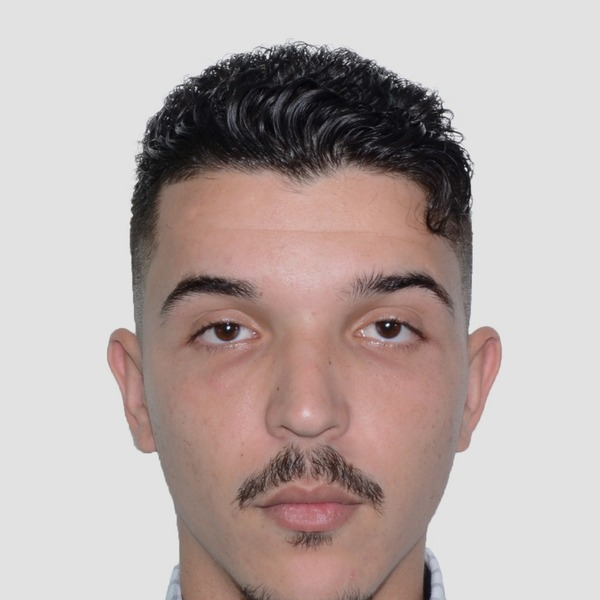
\includegraphics[width=2.3cm]{profile-photo.jpg}%
        };
        \draw[accent, line width=1.2pt] (0,0) circle (1.15cm);
    \end{tikzpicture}%
}

\begin{document}
\normalsize
\setlength{\tabcolsep}{0pt}

% ── Header with photo ───────────────────────────────────────────────────────
\noindent
\begin{minipage}[c]{0.17\textwidth}
    \centering
    \profilephoto
\end{minipage}%
\hfill
\begin{minipage}[c]{0.80\textwidth}
    \cvname{Hamza Bouktitiya}\\[2pt]
    \cvtitle{Artificial Intelligence Engineer \textbullet\ PhD Candidate}\\[4pt]
    \cvmeta{%
        \faMapMarker*\ Kenitra, Morocco
        \quad\textbullet\quad
        \faPhone*\ +212~688~679~653
        \quad\textbullet\quad
        \faEnvelope*\ \href{mailto:bouktitiya.hamza.post@gmail.com}{bouktitiya.hamza.post@gmail.com}
    }\\[2pt]
    \cvmeta{%
        \faLinkedin*\ \href{https://www.linkedin.com/in/hamza-bouktitiya-604471253/}{LinkedIn}
        \quad\textbullet\quad
        \faGithub*\ \href{https://github.com/gothamza}{GitHub}
        \quad\textbullet\quad
        \faGlobe*\ \href{https://gothamza.github.io/portfolio/}{Portfolio}
    }
\end{minipage}

\vspace{2pt}
{\footnotesize\color{ink}
AI engineer and PhD candidate building production LLM systems (RAG, agents, APIs) with FastAPI, LangChain/LangGraph, and Docker. Experience spanning NLP, computer vision, and full-stack deployment.}

% ── Education ───────────────────────────────────────────────────────────────
\section*{Education}
\begin{itemize}
    \item \role{PhD Candidate in Artificial Intelligence}{2024 -- Present}
          \org{Ibn Tofail University, Kenitra, Morocco}
          Thesis: \textit{Textual description and automatic classification of video sequences by deep learning.}
          Supervisor: Prof.\ Housni Khalid.

    \item \role{Master in Artificial Intelligence and Virtual Reality}{2022 -- 2024}
          \org{Ibn Tofail University, Kenitra, Morocco}

    \item \role{Bachelor in Mathematical and Computer Science}{2018 -- 2022}
          \org{Ibn Tofail University, Kenitra, Morocco}

    \item \role{Baccalaureate in Mathematical Sciences}{2017 -- 2018}
          \org{Sidi Aissa High School, Souk El Arbaa Du Gharb}
\end{itemize}

% ── Experience ──────────────────────────────────────────────────────────────
\section*{Professional Experience}
\begin{itemize}
    \item \role{Junior AI Engineer}{April 2025 -- October 2025}
          \org{OBYSTECH SOLUTIONS, Rabat}
          Designed and shipped a multi-department AI agent platform (HR, Finance, Management, IT) as a solo project.
          \begin{itemize}
              \item Built a multi-chat Next.js front end with collection selector, per-chat RAG toggle, team workspaces, and cursor-based pagination.
              \item Implemented a RAG pipeline (PDF/docs ingestion, Hugging Face embeddings, hybrid/vector search with MMR) and LangGraph workflows with PostgreSQL-backed memory; MCP for external tools.
              \item Deployed a multi-service Docker Compose stack on VPS with reverse proxy, SSL, and zero-downtime restarts.
              \item \textbf{Stack:} Next.js, FastAPI, LangChain, LangGraph, MCP, Ollama, PostgreSQL, ChromaDB, Docker, JWT/OAuth2.
          \end{itemize}

    \item \role{AI Intern}{February 2024 -- August 2024}
          \org{Verve Technologie, Casablanca}
          \begin{itemize}
              \item Built an LSTM forecasting system for energy consumption prediction.
              \item Exposed Stable Diffusion~1.5 image-generation endpoints and a RAG pipeline over Wikipedia/PDF sources.
              \item Added JWT authentication and user management on FastAPI.
              \item \textbf{Stack:} LSTM, LangChain, FastAPI, Stable Diffusion, JWT.
          \end{itemize}

    \item \role{Web Development Intern}{March 2022 -- June 2022}
          \org{CS Department, Ibn Tofail University, Kenitra}
          Developed a gym management web app for clients and administrators (PHP, JavaScript, Bootstrap, MySQL).
\end{itemize}

% ── Skills ──────────────────────────────────────────────────────────────────
\section*{Technical Skills}
\begin{tabularx}{\textwidth}{@{}>{\bfseries}l@{\hspace{0.6em}}X@{}}
AI / ML     & PyTorch, TensorFlow, LangChain, LangGraph, CrewAI, RAG, LLMs, NLP, Computer Vision, NeRF \\
Back-end    & FastAPI, Django, Python, REST APIs, PostgreSQL, MySQL, JWT/OAuth2 \\
Front-end   & Next.js, React, TypeScript, Tailwind CSS, HTML/CSS, Streamlit \\
MLOps / Ops & Docker, Docker Compose, Nginx, VPS deployment, Git/GitHub \\
Data        & Pandas, NumPy, Power BI, TF-IDF, classical ML (SVM, KNN) \\
\end{tabularx}

% ── Projects ────────────────────────────────────────────────────────────────
\section*{Selected Projects}
\begin{itemize}
    \item \textbf{Intelligent Assessment System} (2026) --- LLM/RAG platform for exam generation, answer evaluation, and personalized feedback (BLEU, ROUGE, BERTScore); FastAPI, Streamlit, LangChain, Docker.
    \item \textbf{Computer Vision Playground} (2025) --- Dockerized Streamlit app for MTCNN face detection, LBPH recognition, YOLOv8 object detection, and MediaPipe pose estimation.
    \item \textbf{Darija Q\&A System} (2023) --- Bilingual Moroccan Darija/English QA with Transformer QA, Seq2Seq, and LSTM translation models.
    \item \textbf{License Plate Recognition} (2023) --- HOG features with KNN/SVM character classifiers; \textbf{98.9\%} test accuracy.
\end{itemize}

% ── Languages \& Activities ──────────────────────────────────────────────────
\section*{Languages \& Activities}
\textbf{Languages:} Arabic (Native) \textbullet\ English (C1) \textbullet\ French (B2)\\[2pt]
\textbf{Activities:} DyslexAI Hackathon --- Top~3 (Al Akhawayn University) \textbullet\
ThinkAI Hackathon (1337 Coding School) \textbullet\
Co-founder, Pragnomos Club \textbullet\
ML talk at Agora event

\end{document}
